\section{Audit Design}
\label{sec:design}

\Cref{fig:overview} summarizes the audit: three benchmark families with eleven subsystems and a second release of three of them, sixteen methods in three roles, one reference configuration with integrity checks, and the two questions asked of the resulting per-case table.

\begin{figure}[t]
\centering
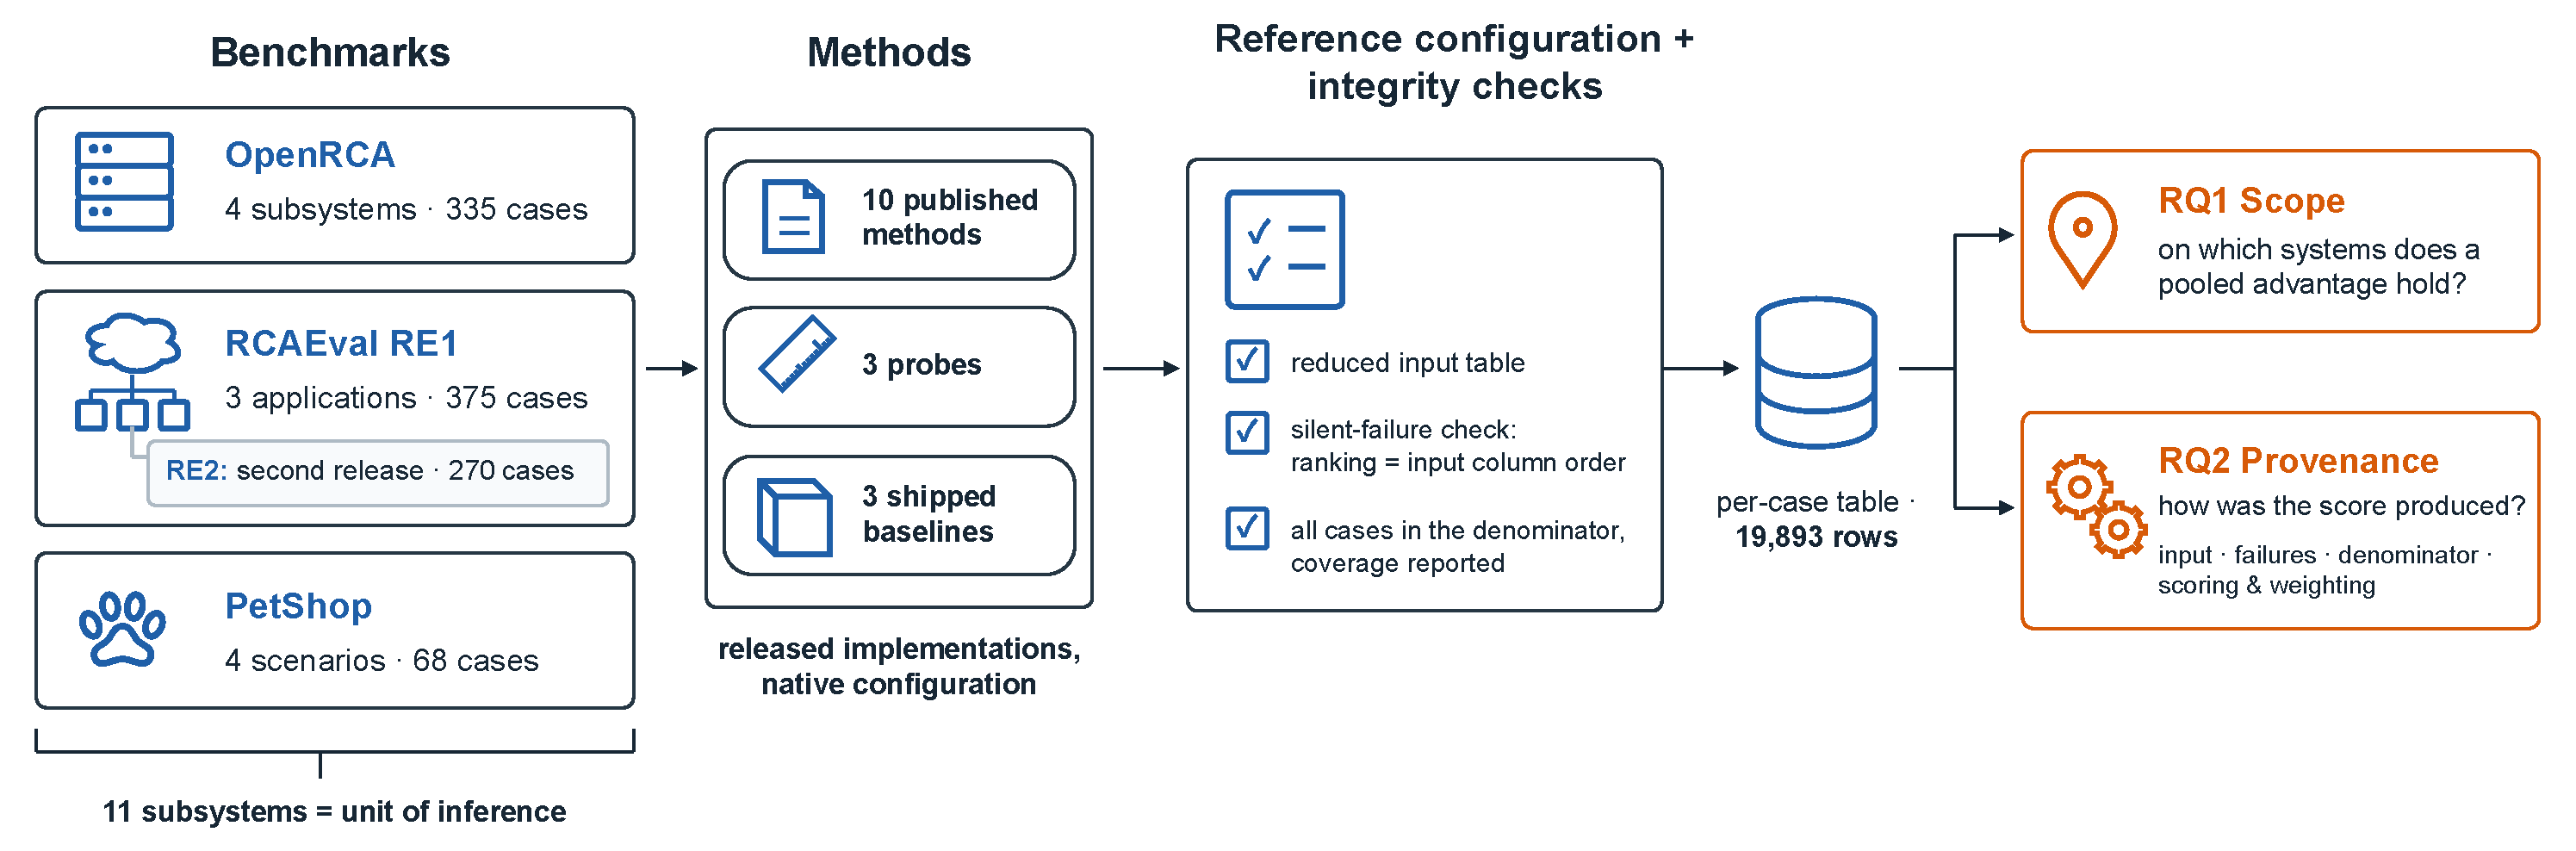
\includegraphics[width=\textwidth]{figures/fig_overview.pdf}
\caption{Overview of the audit. Methods are scored case by case on every subsystem where they run; RQ1 asks on which subsystems a pooled advantage holds, RQ2 which stages of the released evaluation pipeline change it.}
\label{fig:overview}
\end{figure}

\subsection{Benchmarks and Subsystems}
\label{sec:design-bench}

We audit three public benchmark families (\cref{tab:ledger}).
A \emph{subsystem} is one application or scenario inside a family. It is the unit at which an operator would adopt a method, and it is our unit of comparison.

\textbf{\openrca}~\citep{xu2025openrca} contains four subsystems (Bank, Market-1, Market-2, Telecom).
Each query asks for one or more of the root-cause component, the failure reason, and the occurrence time; the official scorer awards the fraction of the required items that match (component and reason by exact string, time within 60\,s).
The audited methods rank metrics, so we wrap them.
A method ranks the metrics of the query window (a 4-hour baseline plus 30 minutes on either side of the window midpoint).
The answer component is the first ranked metric that belongs to the query's candidate set, the reason is mapped from that metric's type, and the time is the moment of largest deviation.
For a query that states $n$ failures, the wrapper returns the first $n$ distinct candidate components.
No published work compares these methods on \openrca, whose own leaderboard ranks LLM agents; the comparison is our construction through this wrapper, and RQ1 reports it separately from the comparisons that exist in the literature.
\cdmin runs on one-minute data with a detection window that ends one minute after the query midpoint, the setting for which it was written.

\textbf{\rcaeval}~\citep{pham2024rcaeval} releases three suites over the same three applications (Online Boutique, Sock Shop, Train Ticket).
RE1 (metrics only; five fault types) provides three subsystems of the main analysis.
RE2 (six fault types; metrics, logs, and traces) is a second, independently collected release of the same applications; we use it only to ask whether conclusions carry over between releases, and do not count it as further subsystems.
The scoring rule is top-1 at service level, a ranked metric mapping to the service named by its prefix, with the benchmark's default window of 20 minutes around the injection time.

\textbf{\petshop}~\citep{hardt2024petshop} provides four traffic scenarios (high traffic, low traffic, and two temporal scenarios), scored by its official harness at node level.

The main analysis thus has $k=11$ subsystems and 778 cases, and each method is scored on every case of the subsystems where it runs; RE2 adds 270 cases.
% src: tab4 n row; coverage.csv n. 335+375+68 = 778; RE2 3x90 = 270

\begin{table}[t]
\caption{Audit ledger. Every method is scored on every case of a subsystem; invalid outputs score 0. RE2 is a second, independently collected release of the RE1 applications and is used only for cross-release comparisons.}
\label{tab:ledger}
\small
\setlength{\tabcolsep}{4pt}
\begin{tabular}{@{}l>{\raggedright\arraybackslash}p{4.3cm}>{\raggedright\arraybackslash}p{3.3cm}ll@{}}
\toprule
Family & Subsystems (cases) & Input used & Scoring & Role \\
\midrule
\openrca & Bank (136), Market-1 (70), Market-2 (78), Telecom (51) & official telemetry & partial credit & main, $k=4$ \\
\rcaeval RE1 & OB (125) & the only shipped table & top-1 service & main, $k=3$ \\
 & SS (125), TT (125) & reduced metric table & top-1 service & \\
\petshop & High (26), Low (26), Temporal-1 (8), Temporal-2 (8) & official harness & top-1 node & main, $k=4$ \\
\rcaeval RE2 & OB, SS, TT (90 each) & reduced metric table, logs, traces & top-1 service & cross-release \\
\bottomrule
\end{tabular}
\end{table}

\subsection{Methods and Their Roles}
\label{sec:design-methods}

Methods enter the audit in one of three roles.
\emph{Published methods} are the objects of the audit: \baro~\citep{pham2024baro}, \circa~\citep{li2022circa}, \ediag~\citep{ediagnosis}, \rcd~\citep{ikram2022rcd}, and \causalrca~\citep{causalrca} on RE1; on RE2 additionally \simplerca~\citep{fang2025simplerca}, \tracerca~\citep{li2021tracerca}, \microrank~\citep{yu2021microrank}, and the multi-source variant of \baro shipped with \rcaeval; on \openrca \baro, \ediag, and \rcd; on \petshop \circa, \rcd, \ediag, \cfa~\citep{budhathoki2022causal}, and \baro.
We run the implementations that the benchmarks ship, at the release current when the audit began; the version is recorded in the replication package.
For \simplerca we use the \rcaeval branch of the authors' released code, which reproduces to two decimals every value the authors report for \simplerca and their \baro baseline on RE2 and on RE3, a third release of the same applications that we do not otherwise use.
On RE1, which provides only metrics, that branch reduces to its \baro-based metric ranking, so we do not count it as a separate method there.

\emph{Probes} are three simple rules that we add to test whether a leaderboard orders even simple alternatives consistently.
\maxz picks the metric with the largest absolute z-score after the fault relative to the pre-fault interval; \alertcount picks the service with the most metrics whose z-score exceeds 3; \cdmin, a threshold detector written for \openrca at one-minute resolution, flags metrics whose post-onset peak exceeds the baseline in both z-score and relative change and ranks components by their largest relative change.
\emph{Shipped baselines} are the traversal, ranked-correlation, and random-walk baselines that \petshop distributes.

Not every method runs on every family.
\microrank and \tracerca need traces, which only RE2-OB and RE2-TT provide.
\causalrca would need an estimated 4,900 GPU-hours on \openrca.
\circa's causal-discovery step fails on \openrca because the metric correlation matrix is singular when there are more metrics than time points, and making it run would mean choosing a metric subset, which changes the method's input.
MicroCause, also shipped with \rcaeval, took more than 10 minutes per case and was not run.
\rcd and \causalrca are randomized; we run three seeds and average each case's score over seeds, except for the \rcd implementation that \petshop ships, which we run once through its harness.

\subsection{Reference Configuration and Integrity Checks}
\label{sec:design-protocol}

A released benchmark can be run in more than one way that is consistent with its documentation, and some of those ways change scores without any visible error.
Before comparing methods we therefore fix a reference configuration and check the outputs it produces; the alternatives set aside here become the conditions of RQ2.

\textbf{Input representation.}
RE1-SS and RE1-TT ship two metric tables per case: a raw export with several hundred to over a thousand columns, and a reduced table with a few dozen to about two hundred.\footnote{The raw export is \texttt{data.csv} (421--439 columns on SS, 1,180--1,446 on TT) and the reduced table \texttt{simple\_data.csv} (58--64 and 199--239 columns). The two tables of a case cover the same time points; the reduced table keeps a few aggregated metrics per service (CPU, memory, workload, latency percentiles, errors), the raw export the per-container series they are derived from. RE1-OB ships a single table of 51--60 columns, which we use. RE2 ships the reduced table \texttt{simple\_metrics.csv}.}
The released runner reads the raw export, and the code that would switch to the reduced table is commented out; the metric counts in the repository's documentation, however, match the reduced table.
The choice matters: \baro's Avg@5 (the metric its authors report) on the reduced tables is 0.960 (SS) and 0.779 (TT), close to the 0.95 and 0.81 that its authors, who also built \rcaeval, report, but 0.576 and 0.261 on the raw exports.
% src: runs/baro/baro_re1-{ss,tt}_{len20,datacsv_len20}.json, Avg@5 from ranks; BARO paper §4.6.1
\baro is the only method whose reported values identify the file in this way, so we take the reduced tables as the reference on these two grounds.
The raw exports remain an equally literal reading of the runner; we keep every method's outputs on them and compare the two conditions in \cref{sec:rq2-input}.

\textbf{Silent failures.}
A method that fails inside the pipeline may still return a complete ranking, and nothing in the output marks it.
We check for the simplest signature of such a failure, a ranking equal to the input column order, and found two sources of it in the audited release.
The first is dependency drift: \causalrca calls a PageRank function that scikit-network removed in version 0.32, the released requirements set only a lower bound on that library, and the resulting exception is caught and the input column order returned.
Under scikit-network 0.33.0, \causalrca's ranking equalled the column order in 30 of 30 cases of a permutation test; under 0.31.0 in 0 of 30, and we run it under that version.
The second is a duplicated column header in 50 of the 125 RE1-OB tables, on which \circa fails and returns the column order, and \ediag ranks the duplicated column first, in 49 cases each.
% src: .research/verifications/2026-09-30-re1ob-duplicate-time-column.md §3
Both are fixed in the current upstream release.
We apply the same fix to the input, rerun the affected methods on the affected cases, and keep the as-shipped outputs for \cref{sec:rq2-defect}.

\textbf{Conventions.}
All RE1 and RE2 methods use the 20-minute default window.
An output is invalid if the method raised an error, returned no candidate, or, on \openrca, the wrapper fell back to a fixed default answer.
Invalid outputs score 0 and the denominator is always the full case set.
We mark every accuracy whose coverage (the share of valid outputs) is below 1 and report the coverage values in \cref{sec:rq2-denominator} and the replication package.
All per-case outputs, each with the configuration of the run that produced it, are merged into one table of \NlongRows rows; after freezing, every analysis reads only this table.

\subsection{Statistics}
\label{sec:design-stats}

For methods $A$ and $B$ on subsystem $s$ with $n_s$ matched cases, the subsystem effect is the mean paired difference $\Delta_s = n_s^{-1}\sum_i (y^A_{s,i} - y^B_{s,i})$, where $y$ is the case score (top-1 hit, or the \openrca partial score).
Its 95\% confidence interval (CI) is a percentile bootstrap over cases within the subsystem ($B = 10{,}000$)~\citep{efron1993bootstrap}.
The \emph{pooled} difference $\bar\Delta$ is the unweighted mean of $\Delta_s$ over the $k$ subsystems of a family, so that each subsystem counts once, and its CI averages the subsystems' bootstrap replicates with the same weights; weighting by cases instead changes the reversal count of \NcwDiff pair only.
The pooled CI describes the evaluated set of subsystems; it makes no claim about a subsystem outside it.
% src: pairs.csv, variant mean: compare n_rev_cw vs n_rev_se

A \emph{point-estimate reversal} is a subsystem whose $\Delta_s$ has the opposite sign of a non-zero pooled difference; a \emph{CI-supported reversal} additionally has its CI entirely on the opposite side of zero.
The pooled difference itself need not exclude zero: a CI-supported reversal says that one subsystem has a nominal 95\% CI entirely on the side opposite to the pooled point estimate.
The CIs are nominal and not adjusted for the number of comparisons (\cref{sec:threats}).
A \emph{sign change} between two conditions includes a difference that becomes or stops being zero.
We also describe each comparison by its \emph{pooled margin} $|\bar\Delta|$ and its \emph{between-subsystem spread}, the sample standard deviation of $\Delta_s$ over the $k$ subsystems.
For families with $k \geq 4$ the replication package also gives a random-effects prediction interval~\citep{inthout2016plea}, with the between-subsystem variance estimated by the Paule--Mandel method and a $t$ distribution with $k-2$ degrees of freedom; with $k=4$ it rests on two degrees of freedom and almost always includes zero, so we draw no conclusion from it.
A case-level test of the method-by-subsystem interaction for every pair is in the replication package.

\emph{Held-out subsystems.}
To ask whether a pooled ranking chooses correctly on a subsystem it has not seen, we hold out each subsystem of a family in turn and rank the methods by their mean over the remaining subsystems.
For every adjacent pair in that ranking we check whether the higher-ranked method is also more accurate on the held-out subsystem.
The \emph{regret} of a pooled winner on subsystem $s$ is the accuracy of the best method on $s$ minus the winner's accuracy there.

\emph{Cross-family set.}
The methods with outputs on all 11 subsystems, \baro, \rcd, \ediag, and the three probes (\XNMethods methods, \XNPairs pairs), are also compared across families; on \petshop, \rcd and \ediag are the implementations \petshop ships, elsewhere those of \rcaeval.
Because \openrca's partial credit and top-1 accuracy are on different scales, we do not average them: across families we ask only whether a pair's subsystem differences have both signs, which does not depend on the scale, and whether that remains so when a family or two subsystems are dropped.

Throughout, we report two layers: comparisons between published methods, which are what a leaderboard is read for, and all pairs including probes and shipped baselines.
The former compare the released implementations as we ran them, not the numbers the original papers report.

\subsection{Use of LLM Tools}
\label{sec:design-llm}

LLM sessions were used to locate the tables, passages, and repository contents behind the checks of \cref{sec:bg-survey}; every statement made there was verified by an author against the paper or the repository.
No LLM produced or scored a method output.
